%!TEX root = ../../report.tex
\subsection{Scenarios}
\copied{Scenarios : The description of an architecture is illustrated using a small set of use cases, or scenarios which become a fifth view. The scenarios describe sequences of interactions between objects, and between processes. They are used to identify architectural elements and to illustrate and validate the architecture design. They also serve as a starting point for tests of an architecture prototype. This view is also known as use case view.\\
\\
Scenarios are putting it all together. Interaction between objects in the
system is expressed by object interaction and scenario diagrams as shown on
Figure 6.
}
{from wikipedia\\\url{https://en.wikipedia.org/wiki/4\%2B1_architectural_view_model} and \url{http://pld.ttu.ee/~kruus/db_is02.pdf}}
This section describes the scenarios that are most likely to happen in our system. Scenarios are the interactions from our system with the different actors. First a textual step by step scenario is given, after that a diagram is shown with the scenario diagram.

\subsubsection*{Flood scenario}
\begin{figure}[hb!]
%\centering
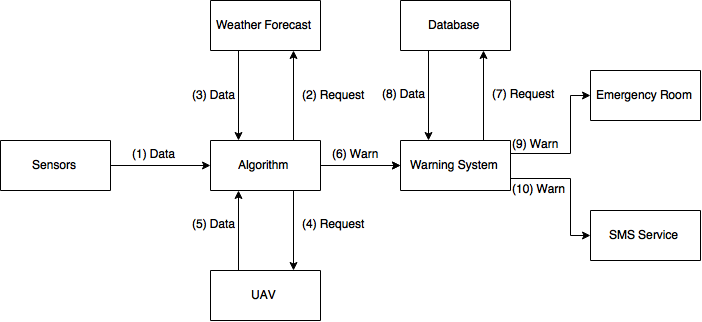
\includegraphics[keepaspectratio=true,width=0.9\textwidth]{{\viewimages/scenario1}.png}
\caption{Scenario for a flood}
\label{fig:layers}
\end{figure}

Main scenarios: \\
1. The sensors monitor the water level \\
%The algorithm determines that the water levels are rising
2. The algorithm requests weather forecast data \\
%The algorithm predicts the probability of a flood
%The probability is above a certain threshold
3. The algorithm sends a warning to the warning part \\
4. The warning part invokes the emergency room API \\
5. The warning part composes a list with phonenumbers that are subscribed and are in the affected area \\
6. The warning part invokes the SMS API, which sends a SMS to all phonenumbers on the list \\\\

A flood is happening or about to happen \\
A citizen needs guidance to a safe area \\
The citizen uses a third party application \\
The third party application gets the current flood information from the third party API \\
The third party application calculates a route to a safe spot \\
The citizen follows the direction and gets into safety
